\documentclass{beamer}
\beamertemplatenavigationsymbolsempty
\usepackage[french]{babel}
\usepackage{fontspec}
\usepackage{amsmath, amsthm, amsfonts}
\usepackage[separate-uncertainty]{siunitx}
\usepackage{xcolor}
\usepackage{tikz}
\usepackage{tikz-cd}
\usepackage[object=vectorian]{pgfornament}
\usepackage{circuitikz}
\usepackage{hyperref}
\usepackage{caption}
\usepackage{booktabs}
\usepackage{mathtools}
\usepackage{longtable}
\usepackage[version=3]{mhchem}
\usepackage{marginnote}
\usepackage[framemethod=tikz]{mdframed}


% Paul Tol's qualitative palette
% ``bright''.https://personal.sron.nl/~pault/#sec:qualitative
\definecolor{tblue}{HTML}{4477AA}
\definecolor{tcyan}{HTML}{66CCEE}
\definecolor{tgreen}{HTML}{228833}
\definecolor{tyellow}{HTML}{CCBB44}
\definecolor{tred}{HTML}{EE6677}
\definecolor{tpurple}{HTML}{AA3377}
\definecolor{tgrey}{HTML}{BBBBBB}


% Justification for marginnotes.
\renewcommand*{\raggedleftmarginnote}{}
\renewcommand*{\raggedrightmarginnote}{}


% Styles for mdframed environments.
\newmdenv[backgroundcolor=tgreen!10,linecolor=tgreen!30]{reponsebox}
\newmdenv[backgroundcolor=tyellow!10,linecolor=tyellow!30]{diapobox}
\newmdenv[backgroundcolor=tred!10,linecolor=tred!30]{fondamentalbox}

% Default arrow for tikz and style for positive and negative objects.
\tikzset{>=latex,
    negative/.style={draw=teal!70!black, fill=teal!10, thick},
    positive/.style={draw=red, fill=red!10, thick}}
\usetikzlibrary{matrix,calc,decorations.pathreplacing,decorations.pathmorphing,decorations.markings}

% French locale for numbers and negative exponent for units.
\sisetup{locale=FR, per-mode=symbol}

\newcommand{\abs}[1]{\left| #1 \right|}
\newcommand{\rhat}{\vec{\hat{r}}}
\newcommand{\xhat}{\vec{\imath}}
\newcommand{\yhat}{\vec{\jmath}}
\newcommand{\zhat}{\vec{k}}
\newcommand{\real}{\mathbb{R}}
\newcommand{\der}[2]{\frac{\mathrm{d}#1}{\mathrm{d}#2}}
\newcommand{\pder}[2]{\frac{\partial\ #1}{\partial\ #2}}
\newcommand{\dif}{\mathrm{d}}
\newcommand{\ddif}{\,\mathrm{d}}
\newcommand{\grad}{\vec{\nabla}}
\newcommand{\exemple}[1]{\begin{fullwidth}#1\end{fullwidth}}
\newcommand{\norm}[1]{\lVert\ #1\ \rVert}
\newcommand{\vu}{\vec{u}}
\newcommand{\vv}{\vec{v}}
\newcommand{\vr}{\vec{r}}
\newcommand{\va}{\vec{a}}
\newcommand{\vF}{\vec{F}}
\newcommand{\vE}{\vec{E}}
\newcommand{\vB}{\vec{B}}
\newcommand{\vecxyz}[3]{#1 \xhat\ + #2 \yhat\ + #3 \zhat}
\newcommand{\vecxy}[2]{#1 \xhat\ + #2 \yhat}
\newcommand{\coulombcst}{k}
\newcommand{\emf}{\ensuremath{\mathcal{E}}}
\newcommand{\eval}{\SI{1.602e-19}{C}}
\newcommand{\kval}{\SI{8.99e9}{Nm^2 \per C^2}}

% Nice separator line
\newcommand{\sectionline}{
    \noindent
    \begin{center}
        \resizebox{0.5\linewidth}{1ex}
    {{%
    {\begin{tikzpicture}
    \node  (C) at (0,0) {};
    \node (D) at (9,0) {};
    \path (C) to [ornament=85] (D);
    \end{tikzpicture}}}}
    \end{center}
}

\theoremstyle{definition}
\newtheorem*{defn}{Definition}


\usepackage[version=3]{mhchem}

\setbeamercolor{title}{fg=tblue}
\setbeamercolor{frametitle}{fg=tblue}
\setbeamercolor{structure}{fg=tblue}

\title{Électricité et magnétisme}
\subtitle{Chapitre 1 - Charge électrique}
\date{25 août 2021}
\author{Loïc Séguin-Charbonneau}
\institute{Cégep Édouard-Montpetit}

\begin{document}

\maketitle

\begin{frame}{Capacité d'une batterie de téléphone}
\begin{columns}
  \column{0.6\textwidth}
  Un téléphone d'une marque connue a une batterie d'une capacité de \SI{6556}{C}.
  Combien d'électrons peuvent être déplacés par cette batterie?

  \begin{enumerate}[A.]
    \item Environ \num{1e-23}
    \item Environ \num{1e-15}
    \item Environ 6556
    \item<alert@2> Environ \num{1e23}
  \end{enumerate}

  \column{0.4\textwidth}
  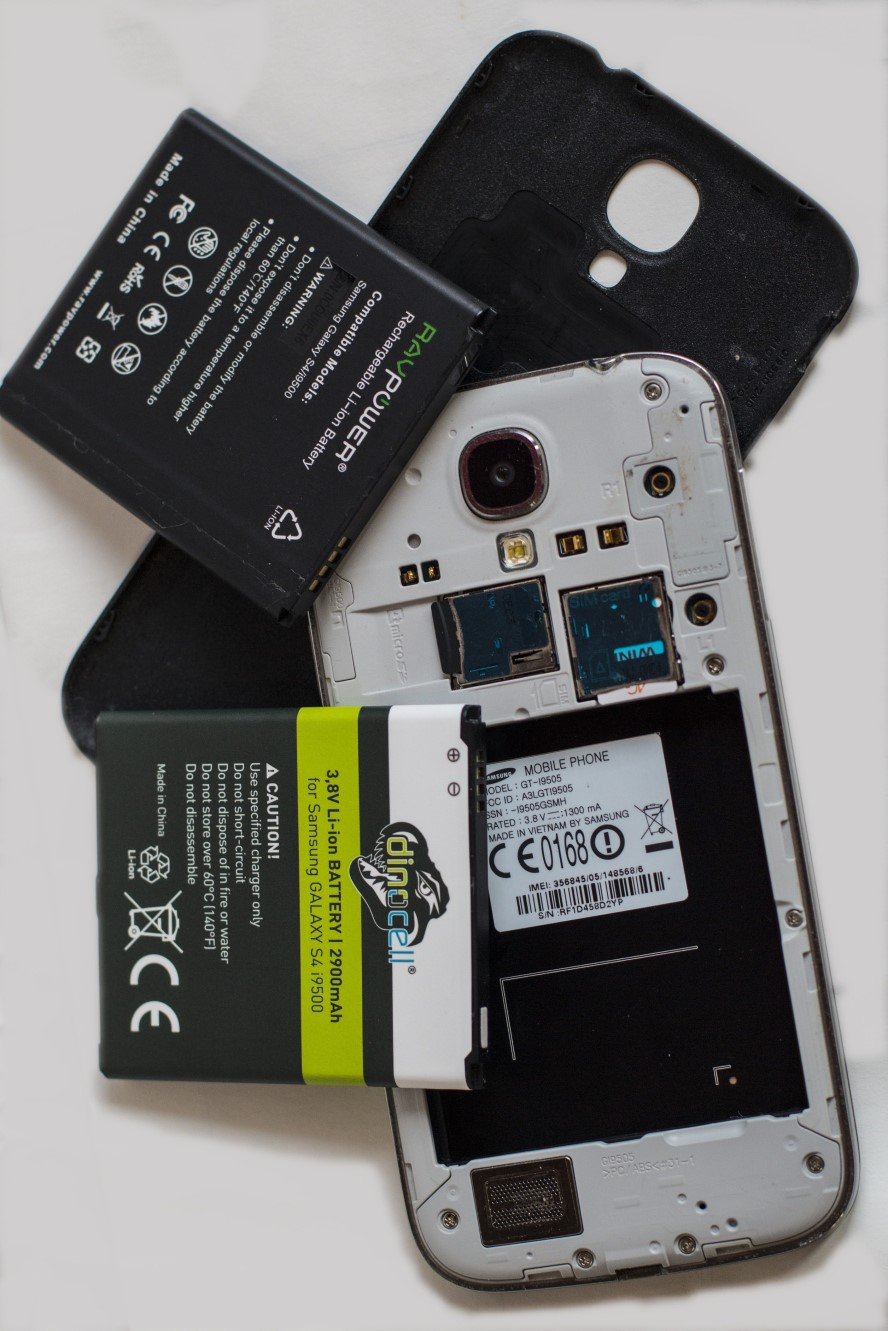
\includegraphics[width=\textwidth]{figures/batterie-telephone.jpg}
\end{columns}
\end{frame}


\begin{frame}{Fission nucléaire}
\begin{columns}
  \column{0.6\textwidth}
  Dans un réacteur nucléaire typique, un neutron lent entre en collision avec un
  noyau d'uranium ce qui provoque la fission du noyau en deux noyaux plus petits:
  \begin{center}
    \ce{n + ^235U -> 3n + ^141Ba + ^AX}
  \end{center}
  Quel est le noyau \ce{^AX}?

  \begin{enumerate}[A.]
    \item \ce{^84Kr}
    \item<alert@2> \ce{^92Kr}
    \item \ce{^94Nb}
    \item \ce{^244Pu}
  \end{enumerate}

  \column{0.4\textwidth}
  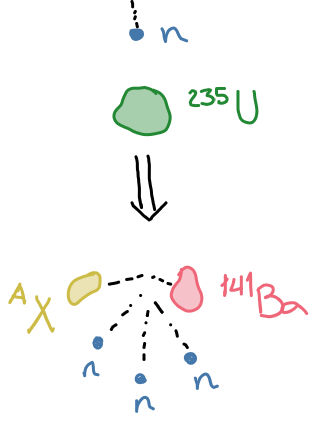
\includegraphics[width=\textwidth]{figures/fission.png}
\end{columns}
\end{frame}


\begin{frame}{Conservation de la charge}
  Indiquez si chacune des réactions suivantes est possible.

  \begin{enumerate}[A.]
    \item \ce{H^+ + OH^- -> H_2O} \only<2>{\alert{oui}}
    \item $\pi^+ + p^+ \longrightarrow \Sigma^0 + K^+$ \only<2>{\alert{non}}
    \item \ce{^4_2He^{2+} + ^14_7N -> ^17_8O + p^+} \only<2>{\alert{non}}
  \end{enumerate}
\end{frame}


\begin{frame}{Quantification de la charge}
  Est-ce qu'un objet peut avoir les charges suivantes?
  \begin{enumerate}[A.]
    \item $q_0 = \SI{0.452e-19}{C}$  \only<2>{\alert{non}}
    \item $q_1 = \SI{-2.05056e-17}{C}$ \only<2>{\alert{oui}}
    \item $q_2 = \SI{3.74868e-18}{C}$ \only<2>{\alert{non}}
    \item $q_3 = \SI{4.00}{C}$ \only<2>{\alert{oui}}
  \end{enumerate}
\end{frame}


\begin{frame}{Attraction par induction dans un conducteur}
  On induit une séparation de charge dans une tige métallique en approchant une
  tige de plastique chargée. Comment sont disposées les charges dans la tige
  métallique?
  \begin{center}
    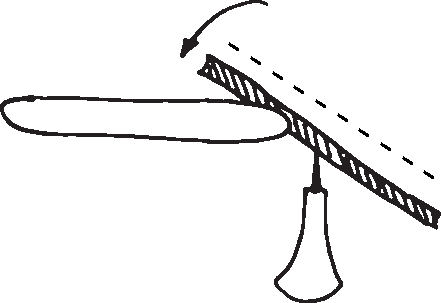
\includegraphics[scale=0.5]{figures/tige-chargee.pdf}
  \end{center}
  \vspace{0.5cm}

  \begin{enumerate}[A.]
    \item 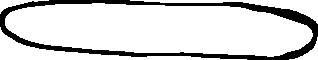
\includegraphics[scale=0.5]{figures/tige.pdf}
      \hspace{-1.3cm}\tikz \node at (-10, 0) {$---$};
    \item 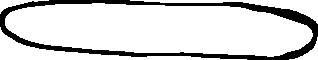
\includegraphics[scale=0.5]{figures/tige.pdf}
      \hspace{-1.3cm}\tikz \node at (-10, 0) {$+++$};
      \hspace{-2.8cm}\tikz \node at (-10, 0) {$+++$};
    \item 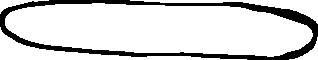
\includegraphics[scale=0.5]{figures/tige.pdf}
      \hspace{-1.3cm}\tikz \node at (-10, 0) {$---$};
      \hspace{-2.8cm}\tikz \node at (-10, 0) {$+++$};
    \item 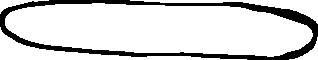
\includegraphics[scale=0.5]{figures/tige.pdf}
      \hspace{-1.3cm}\tikz \node at (-10, 0) {$+++$};
    \item<alert@2> 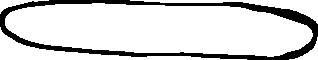
\includegraphics[scale=0.5]{figures/tige.pdf}
      \hspace{-1.3cm}\tikz \node at (-10, 0) {$+++$};
      \hspace{-2.8cm}\tikz \node at (-10, 0) {$---$};
  \end{enumerate}
\end{frame}


\begin{frame}{Électroscope}
  Que se passe-t-il si on touche la partie du haut avec une
  tige chargée négativement puis qu'on la retire?

  \begin{enumerate}[A.]
    \item Les feuillets de l'électroscope s'éloignent puis reviennent à leur
      position initiale.
    \item Les feuillets de l'électroscope se rapprochent puis reviennent à leur
      position initiale.
    \item<alert@2> Les feuillets de l'électroscope s'éloignent et demeurent éloignés.
    \item Les feuillets de l'électroscope se rapprochent et demeurent
      rapprochés.
    \item Les feuillets de l'électroscope demeurent immobiles.
  \end{enumerate}
\end{frame}


\begin{frame}[t]{Exercice}
\begin{columns}
  \column{0.7\textwidth}
  Deux fourchettes métalliques identiques ont des charges $Q$ et $-6Q$,
  respectivement. Les deux fourchettes sont mises en contact puis sont
  séparées.  Quelles sont les charges sur chacune des fourchettes?

  \vspace{\baselineskip}
  \textit{Justifiez votre réponse à partir des principes fondamentaux et des
  définitions.}

  \column{0.3\textwidth}
  \begin{center}
    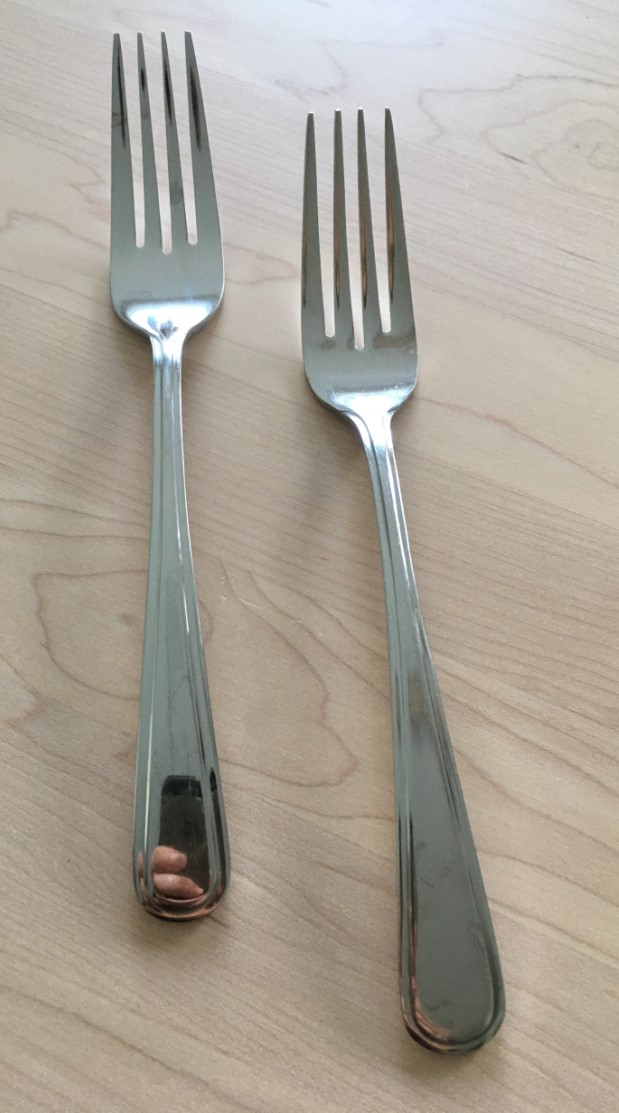
\includegraphics[width=\textwidth]{figures/fourchettes.jpg}
  \end{center}
\end{columns}
\end{frame}


\begin{frame}{Ballon au mur}
Le coefficient de frottement entre le mur et le ballon est $\num{0.6}$, et la
masse du ballon est de \SI{2.9}{g}. Quel est le module de la force électrique
entre le ballon et le mur?
\begin{center}
  \begin{tikzpicture}
    \draw (3, 1.7) -- (3, -1.9);
    \draw (2.298, -1.928) arc (-40:40:3);
    \draw[decorate, decoration={markings,
      mark=between positions 0 and 1 step 8mm with {
        \node[circle, negative, minimum size=4mm] (0, 0) {$-$};}}]
    (1.915, -1.607) arc (-40:40:2.5);
    \foreach \y in {1.7, 0.9, 0.1, -0.7, -1.5} {
      \draw[positive] (3.7, \y) arc (90:270:0.5 and 0.3) -- (3.7, \y);
      \node at (3.5, \y - 0.3) {$+$};
      \draw[negative] (3.71, \y - 0.6) arc (-90:90:0.5 and 0.3) -- (3.71, \y - 0.6);
      \node at (3.9, \y - 0.3) {$-$};
    }
    \coordinate (origin) (0, 0);
    \draw<2>[ultra thick, ->] (origin) -- (-1, 0) node[left] {$\vec{N}$};
    \draw<2>[ultra thick, ->] (origin) -- (1, 0) node[right] {$\vec{F}_e$};
    \draw<2>[ultra thick, ->] (origin) -- (0, 1.4) node[right] {$\vec{f}$};
    \draw<2>[ultra thick, ->] (origin) -- (0, -1.4) node[right] {$\vec{F}_g$};
    \draw[draw=white,fill=white] (-0.02, -0.02) rectangle (0.02, 0.02);
    \node at (-1, 1.7) {Ballon};
    \node at(6, 1.7) {Mur};
  \end{tikzpicture}
\end{center}
\end{frame}


\begin{frame}{Passage d'électrons}
  Vous vous tenez à \SI{2}{m} de votre ami. Combien d'électrons devez vous lui
  transférer pour que la force électrique entre vous deux soit égale à votre
  poids?
  \begin{center}
    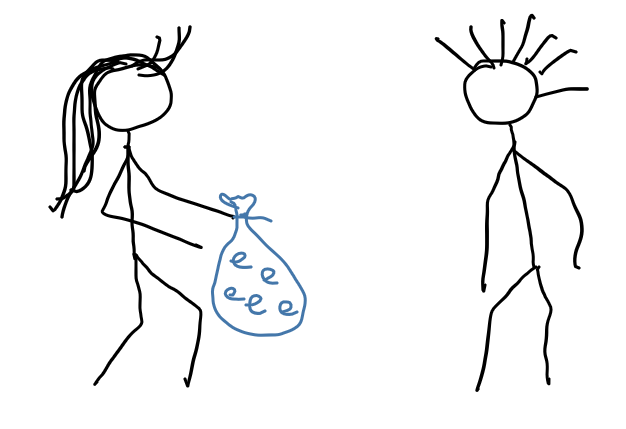
\includegraphics[scale=0.5]{figures/passage-electrons.png}
  \end{center}
\end{frame}


\begin{frame}{Direction des vecteurs}
  On considère une charge négative $q_1$ et une charge positive $q_2$.
  \begin{center}
    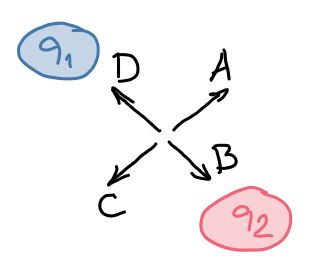
\includegraphics[scale=0.5]{figures/coulomb-direction.png}
  \end{center}

  Dans quelle direction est la force de $q_1$ sur $q_2$, $\vF_{2 \leftarrow 1}$?
  \pause

  Dans quelle direction est la force de $q_2$ sur $q_1$, $\vF_{1 \leftarrow 2}$?
  \pause
  
  Dans quelle direction est le vecteur $\vu_{1 \rightarrow 2}$?
  \pause

  Dans quelle direction est le vecteur $\vu_{2 \rightarrow 1}$?
\end{frame}


\begin{frame}{Interaction transmembranaire}
\begin{columns}
  \column{0.6\textwidth}
    Un ion \ce{Na+} et un ion \ce{PO4^3-} se trouvent de part et d'autre d'une
    membrane cellulaire. L'épaisseur de la membrane est de \SI{5}{nm} et les
    deux ions sont décalés de \SI{10}{nm} l'un par rapport à l'autre le long de
    la membrane. Quelle est la force exercée par le sodium sur le phosphate?

  \column{0.4\textwidth}
  \begin{center}
    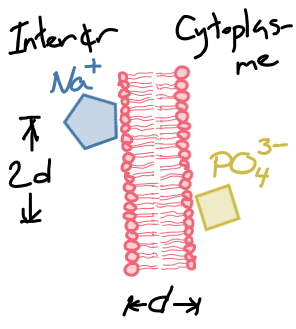
\includegraphics[scale=0.5]{figures/exercice-membrane.png}
  \end{center}
\end{columns}
\end{frame}


\begin{frame}{Coulomb 1D}
  Deux charges immobiles $q = \SI{4.00}{nC}$ et $Q = \SI{-6.00}{nC}$ sont
  situées à \SI{5}{cm} l'une de l'autre.  Où doit-on positionner une troisième
  charge de telle sorte qu'elle soit à l'équilibre?
  \begin{center}
    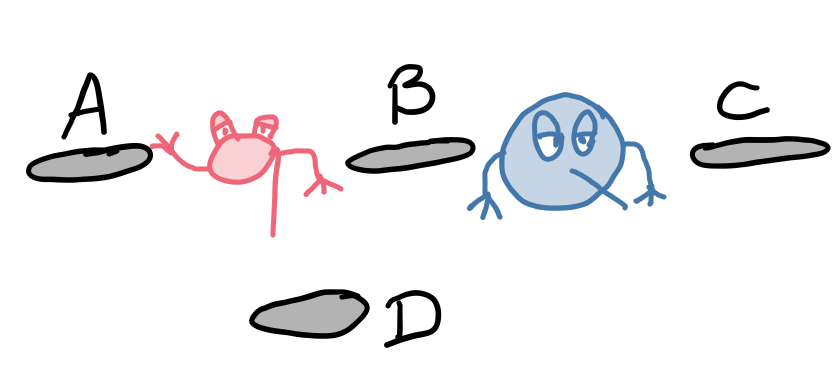
\includegraphics[scale=0.4]{figures/petitq-grosq.png}
  \end{center}
\end{frame}



\end{document}
